%! Author = sriadityavedantam
%! Date = 4/7/26

\section{Zarisky Topologies on Projective Varieties}

Take a Zariski closed subset $X\subset \pp^n$.
These correspond one-to-one with radical homogeneous ideals
\[
    I\subset \kk[\reptiln{x}{n+1}].
\]
Thus we need the notion of a homogeneous ideal.

\begin{definition}[Homogeneous Ideal]
    Take a graded ring
    \[
        R = \bigoplus_{d=0}^{\infty} R_d
    \]
    and an ideal $I\subset R$.
    We say $I$ is homogeneous if for every $f\in I$, when we write
    \[
        f = f_0 + f_1 + \cdots + f_d
    \]
    with each $f_i\in R_i$, then each homogeneous piece $f_i$ also lies in $I$.
    Equivalently, $I$ is generated by homogeneous elements.
\end{definition}

\begin{definition}[Canonical]
    A subset is canonical if it is closed under scalar multiples along lines through the origin.
\end{definition}

\begin{lemma*}{
    If $p(\reptiln{x}{n+1})$ is a homogeneous polynomial of degree $d$, then on the affine chart $x_0\neq 0$ there is a corresponding polynomial
    \[
        q(\reptiln{y}{n}) = p(1,\reptiln{y}{n}).
    \]
    Conversely, given a polynomial $q(\reptiln{y}{n})$ of degree at most $d$, the associated homogeneous polynomial is
    \[
        x_0^d q\left(\frac{x_1}{x_0},\ldots,\frac{x_n}{x_0}\right).
    \]
}
\end{lemma*}

If we take
\[
    q(y_1,y_2) = y_1^2 + y_2^2 - 4,
\]
then its homogeneous lift is
\[
    x_0^2\left(\left(\frac{x_1}{x_0}\right)^2 + \left(\frac{x_2}{x_0}\right)^2 - 4\right)
    = x_1^2 + x_2^2 - 4x_0^2.
\]

Then
\[
    \pp^2\setminus \aa^2 = \{x_0 = 0\},
\]
which is the line at infinity.

\begin{lemma*}{
    The Zariski topology on $\pp^n$ restricted to the chart $\aa^n$ is the Zariski topology on $\aa^n$.
}
\end{lemma*}

\begin{remark}
    Look at the following diagram.
\end{remark}

\begin{figure}[H]
    \centering

    \tikzset{every picture/.style={line width=0.75pt}}

    \colorbox{white}{%
        \color{black}
        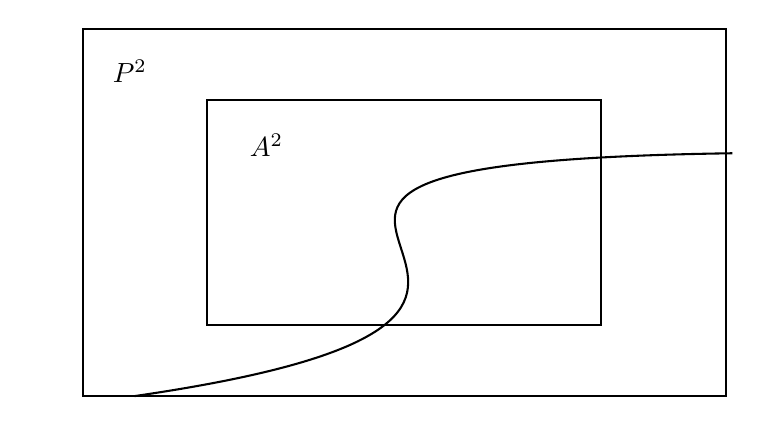
\begin{tikzpicture}[
            x=0.75pt,
            y=0.75pt,
            yscale=-1,
            xscale=1,
            every node/.style={text=black},
            every path/.style={draw=black},
            line width=0.75pt
            ]
                \draw   (174,45) -- (483.75,45) -- (483.75,222) -- (174,222) -- cycle ;
                \draw   (233.88,79.21) -- (423.88,79.21) -- (423.88,187.79) -- (233.88,187.79) -- cycle ;
                \draw    (199,222) .. controls (495,179) and (148,110) .. (487,105) ;

                \draw (253,94.4) node [anchor=north west][inner sep=0.75pt] {$\mathbb{A}^{2}$};
                \draw (187,58.4) node [anchor=north west][inner sep=0.75pt] {$\mathbb{P}^{2}$};
        \end{tikzpicture}
    }
\end{figure}

Now the question is whether this is open or closed.
In fact, the image of a projective variety under a morphism of algebraic varieties is closed in the Zariski topology.
If $Y\subset \aa^n$, then its projective closure $\bar{Y}\subset \pp^n$ satisfies
\[
    I_+(\bar{Y}) = \{\hom(p) : p\in I(Y)\},
\]
where $\hom(p)$ denotes the homogenization of $p$.
We have previously defined affine varieties as Zariski closed subsets of $\aa^n$.
Now take quasi-affine varieties by starting with an affine variety and removing a closed subset.
Thus they are locally closed.
Similarly, we have projective and quasi-projective varieties.

\begin{lemma*}{
    If $U\overset{\text{open}}{\subset} X\overset{\text{closed}}{\subset} \pp^n$ is quasi-projective, then a function $f:U\to \kk$ is regular if for every point $V\in U$ there is a neighborhood on which $f$ is a quotient of homogeneous polynomials of the same degree, with denominator nonzero at $V$.
}
\end{lemma*}

\begin{lemma*}[Sheaf Property]{
    If $Y\subset \aa^n$ is an affine variety, then the set of regular functions agrees with the earlier definition.
    Moreover, the ring of regular functions on $D(f)\subset Y$ is
    \[
        \kk[Y]\left[\frac{1}{f}\right].
    \]
}
\end{lemma*}

\begin{definition}[Sheaf]
    A sheaf is a collection of local regular functions that are compatible on overlaps.
\end{definition}

Maps between quasi-projective varieties are regular maps
\[
    f:U_1\to U_2
\]
such that for each point $v\in U_1$, there is a neighborhood on which $f$ is given by homogeneous polynomials of the same degree:
\[
    f(\reptiln{x}{n+1}) = (p_0(\reptiln{x}{n+1}), \ldots, p_m(\reptiln{x}{n+1})),
\]
and at least one $p_i(v)\neq 0$.

\begin{corollary}{
    Given
    \[
        D(f) = \{f\neq 0\}\subset Y,
    \]
    the open subset $D(f)$ is isomorphic to an affine variety.
}
\end{corollary}

\begin{lemma*}{
    Suppose $U = X\setminus Z\subset \pp^n$ is irreducible.
    Then $U$ is not the union of two proper closed subsets.
    Equivalently, if $W_1,W_2\subset U$ are nonempty open subsets, then
    \[
        W_1\cap W_2\neq \varnothing.
    \]
    The rational functions on $U$ form a field, denoted $\kk(U)$.
}
\end{lemma*}

\begin{lemma*}{
    There is a correspondence
    \[
        \{\text{affine varieties over $\kk$}\}/\text{isomorphism}
        \leftrightarrow
        \{\text{finitely generated $\kk$-algebras without nilpotents}\}.
    \]
    Similarly,
    \[
        \{\text{quasi-projective irreducible varieties}\}/\text{birational isomorphism}
        \leftrightarrow
        \{\text{finitely generated fields }K/\kk\}.
    \]
}
\end{lemma*}

\begin{definition}[Rational Map]
    A rational map is a regular map defined on a nonempty open subset.
\end{definition}

A famous example is the map
\[
    \pp^1 \to \pp^3
\]
defined by
\[
    (x_0,x_1)\mapsto (x_0^3,x_0^{2}x_1,x_{0}x_1^2,x_1^3).
\]